% ########################################

\chapter{Scheduling Observations}
\label{chap:scheduling}

% ~~~~~~~~~~~~~~~~~~~~

\chaptoc{}

% ########################################

\section{Introduction}
\label{sec:scheduling_intro}

% ~~~~~~~~~~~~~~~~~~~~

\begin{colsection}

Completing the chapters describing the core functions of the GOTO Telescope Control System, in this chapter I detail how the robotic system decides which targets to observe.
%
\begin{itemize}
    \item In \nref{sec:ranking} I describe the functions used by the G\nobreakdash-TeCS scheduler to chose between targets and decide which is the highest priority.
    \item In \nref{sec:scheduler_tiebreaker} I examine how the ``tiebreak'' value is calculated to sort between equally-ranked targets.
    \item In \nref{sec:scheduler_sims} I describe how optimal tiebreak weighting parameters were determined, by running simulations of the G-TeCS system observing gravitational-wave events.
\end{itemize}
%
All work described in this chapter is my own unless otherwise indicated. The first two sections are based on the description of the scheduling functions in \citet{Dyer}.

\end{colsection}

% ########################################

\section{Determining target priorities}
\label{sec:ranking}

% ~~~~~~~~~~~~~~~~~~~~

\begin{colsection}

GOTO operates under a ``just-in-time'' scheduling model \citep[see, for example,][]{LCO_scheduling}, rather than creating a plan at the beginning of the night of what to observe \citep[see, for example,][]{ZTF_scheduler}. Each time the pilot queries the scheduler the current queue of pointings is imported and the priority of each is calculated, with no explicit consideration for the past or future (aside from the ``mintime'' constraints, as described below). The highest priority pointing is then returned, as described in \aref{sec:scheduler}.

This system is very reactive to any incoming alerts, as the new pointings will immediately be included in the queue at the next check. This method also naturally works around any delay in observations due to poor conditions, unlike a fixed night plan. The just-in-time method can be less efficient than a night plan when observing predefined targets which can be deliberately optimised before the night starts. However the just-in-time system is perfectly reasonable for the all-sky survey GOTO is normally observing, and any other observations will be alerts entered by the sentinel daemon which could not be planned for, so it was determined to be the best option for GOTO.\@

Each time the scheduler functions are called several steps need to be carried out. The first of these is to fetch the current queue from the observation database (see \aref{sec:obsdb}). This is done by querying the database \code{pointings} table for any entries that have the \code{pending} status. Additional filters are also applied in order to reduce the number of invalid pointings imported: restricting the query to pointings within the visible region of the sky (based on the time and observatory location) and within the pointing's valid period (the start time has passed and stop time has not yet been reached). Any entries in the table that pass these filters make up the \emph{pointings queue}.

In order to find which pointing is the highest priority, the queue is sorted using a variety of parameters, with the pointing sorted at the top being returned by the scheduler. The sorting criteria are outlined in the following sections.

\end{colsection}

% ~~~~~~~~~~~~~~~~~~~~

\subsection{Applying target constraints}
\label{sec:constraints}
\begin{colsection}

The first consideration is determining which pointings are currently valid. As described in \aref{sec:obsdb}, pointings have limits defined for physical constraints (minimum target altitude, minimum Moon separation, maximum Moon illumination, maximum Sun altitude). These constraints are calculated and applied to the pointings using the Astroplan Python package \citep[\pkg{astroplan}\footnote{\url{https://astroplan.readthedocs.io}},][]{astroplan}. The target altitude and Moon separation constraints depend on the position of the target, both the altitude constraints depend on the site the observations are being taken from, and all four constraints depend on the current time. Each constant is applied both at the current time and after the minimum observing time defined for each pointing. This ensures that, for example, targets that are setting are visible throughout their observing period by checking the altitude is above the minimum both at the beginning and end of the observation. The minimum time constraints are not applied to the pointing currently being observed (if any), as the pointing will already be part way through and will have already been passed as valid. The validity of the pointings is a simple boolean flag (True or False), and invalid pointings are naturally sorted below valid ones.

\end{colsection}

% ~~~~~~~~~~~~~~~~~~~~

\subsection{Effective rank}
\label{sec:rank}
\begin{colsection}

The next order pointings are sorted by is the effective rank of the pointing, which is a combination of the integer starting rank the pointing was inserted with and the number of times it has since been observed.

The starting rank is fixed when the pointing is created in the observation database: every pointing is given an integer rank between 0 and 999. The highest and lowest ranks are reserved for particular classes of targets. Rank 0 is not intended to be used under normal circumstances: it is reserved for exceptional events, such as a local galactic supernova, as a pointing with rank 0 would outrank all other pointings including even gravitational-wave events. At the other end of the scale, rank 999 is reserved for the all-sky survey tiles, so that they are sorted below all other pointings. These pointings act as ``queue fillers'' in the system, ensuring there is always something for the telescope to observe. All other ranks are otherwise available, although by convention ranks ending in 1--5 are used for gravitational-wave events, 6--8 for other transient events (e.g. GRBs) and 9 for other fixed targets. See \aref{sec:event_strategy} for the details of determining the rank for different transient events.

Added to the starting rank is a count of the number of times that a target has been observed, based on the number of pointings previously associated with a given mpointing (see \aref{sec:obsdb}). This count only includes successful observations, so pointings that were interrupted or aborted are not included. The starting rank ($R_s$) and observation count ($n_\text{obs}$) are added to create the effective rank $R$ given by
%
\begin{equation}
    R = R_s + 10\times n_\text{obs}.
    \label{eq:effective_rank}
\end{equation}
%
This formula means a pointing with a starting rank of 2 that has been observed five times will have an effective rank of 52. Effective ranks are sorted in reverse order, so a rank-5 pointing that has been observed once (an effective rank of 15) will be a higher priority target than a rank-4 pointing that has been observed twice (an effective rank of 24). This system allows for a natural filtering of targets, as targets will move down the queue as they are observed. For example, pointings from a gravitational-wave event might be inserted into the database at rank 2, so will first appear in the queue with effective rank of $R=2$ ($n_\text{obs}=0$). The first pointing that is observed will reappear with $R=12$, and therefore be sorted below those tiles that have not yet been observed. Once all the pointings have been observed once they will all have effective rank 12 and the process repeats, with each pointing falling to effective rank 22, 32 etc. As the increase is by 10 each time pointings from other events, or which were manually inserted, might also be in the queue and interweave between the event follow-up pointings. For example, a manual observation might be inserted at rank 9, meaning it will fall below the first observation of the gravitational-wave tiles at $R=2$ but will take priority over subsequent observations. To prevent this, the manual observation could be inserted at rank 19 to come after two gravitational-wave observations, or even 509 to completely ensure it does not interfere with the gravitational-wave follow-up targets.

\end{colsection}

% ~~~~~~~~~~~~~~~~~~~~

\subsection{Targets of Opportunity}
\label{sec:toos}
\begin{colsection}

For pointings with the same effective rank the next sorting parameter is the \acro{too} flag assigned to the pointing when it was inserted into the database. The flag is simply a boolean value that is true if the target is a ToO and false if it is not, and pointings that have the flag as true are sorted higher than those of the same rank that are not ToOs. This ensures that time-sensitive targets are prioritised ahead of other targets at the same rank, although it is important to remember that the effective rank does still take priority (this means a ToO at rank 4 will be sorted above any other rank 4 pointings, but will still be a lower priority than a non-ToO at rank 3).

\end{colsection}

% ~~~~~~~~~~~~~~~~~~~~

\subsection{Breaking ties}
\label{sec:breaking_ties}
\begin{colsection}

Finally, if there are multiple pointings with the same values for the above parameters then a single \emph{tiebreak} value is calculated for each. This value is based on the current airmass of the pointing and the weighting of the survey tile the pointing is linked to, if any; pointings at lower airmass (closer to the zenith) and higher tile weightings are the higher priority. For example, if two new gravitational-wave pointings with equal ranks both contain the same skymap probability (see \aref{sec:skymaps}), then the one at the lower airmass at the time of the check will be prioritised.

\newpage

To calculate the tiebreak value, both the tile weighting ($W$) and airmass ($X$) values need to be scaled between 0 and 1. This is true by definition for the tile weights, while the airmass is scaled so airmasses 1 and 2 are set to 1 and 0 respectively (airmasses greater than 2 are set to zero). The parameters are then combined to form the tiebreak value $V$ in a ratio 10:1 using
%
\begin{equation}
    V = \frac{10}{11}~W + \frac{1}{11}~(2 - X).
    \label{eq:tiebreak}
\end{equation}
%
This ensures the tiebreak value is also between 0 and 1, with higher values being preferred. The best possible scenario is a tile which contains 100\% of the skymap localisation probability ($W=1$) and is exactly at zenith ($X=1$) which gives a tiebreak value $V=1$. How this tiebreak formula was determined is described in \aref{sec:scheduler_tiebreaker}. Note that \aref{eq:tiebreak} is just \aref{eq:wa_ratio} using a ratio of 10:1, which was determined based on the scheduling simulations described in \aref{sec:scheduler_sims}.

In the unlikely event that two pointings are still tied, all other parameters (rank, ToO flag) being otherwise equal, and they have exactly the same tiebreak value, then whichever was inserted into the database first (and therefore has a lower database ID) by default comes first in the queue.

\end{colsection}

% ~~~~~~~~~~~~~~~~~~~~

\subsection{Queue sorting example}
\label{sec:sorting_example}
\begin{colsection}

\begin{table}[t]
    \begin{center}
        \begin{tabular}{c|l|c|ccc|c|ccc} % chktex 44
            & Name & Valid & $R_s$ & $n_\text{obs}$ & Eff.\ rank & ToO & $W$ & $X$ & Tiebreaker \\
            \midrule
            1 & GW191202 P3   & \textcolor{Green}{Y} &  2  & 0 &   2 & \textcolor{Green}{Y} & 0.10 & 1.1 & 0.173 \\
            2 & GW191202 P4   & \textcolor{Green}{Y} &  2  & 0 &   2 & \textcolor{Green}{Y} & 0.05 & 1.1 & 0.127 \\
            3 &         M101  & \textcolor{Green}{Y} &  9  & 0 &   9 &   \textcolor{Red}{N} &    1 & 1.5 & 0.955 \\
            4 & GW191202 P2   & \textcolor{Green}{Y} &  2  & 1 &  12 & \textcolor{Green}{Y} & 0.30 & 1.1 & 0.355 \\
            5 &   AT 2019xyz  & \textcolor{Green}{Y} &  6  & 2 &  26 & \textcolor{Green}{Y} &    1 & 1.4 & 0.964 \\
            6 &          M31  & \textcolor{Green}{Y} &  16 & 1 &  26 &   \textcolor{Red}{N} &    1 & 1.2 & 0.982 \\
            7 & All-sky T0042 & \textcolor{Green}{Y} & 999 & 0 & 999 &   \textcolor{Red}{N} &    1 & 1.0 & 1.000 \\
            \vdots & & & & & & \\
              &  GW191202 P1  &   \textcolor{Red}{N} &   2 & 0 &   2 & \textcolor{Green}{Y} & 0.55 & 1.1 & 0.582 \\
              & All-sky T0123 &   \textcolor{Red}{N} & 999 & 0 & 999 &   \textcolor{Red}{N} &    1 & 2.0 & 0.909 \\
        \end{tabular}
    \end{center}
    \caption[Examples of sorting pointings by priority]{
        Some examples of a queue of pointings sorted by priority. Pointings are first sorted by validity, with invalid pointings shown at the bottom of the queue. Then pointings are sorted by effective rank, which is comprised of the starting rank ($R_s$) and the observation count ($n_\text{obs}$). Pointings with the same effective rank are sorted based on if they are targets of opportunity or not, with ToOs being ranked higher. Finally pointings with all other factors being equal are ranked by the tiebreaker value, combining tile weighting ($W$) and the current airmass ($X$) using \aref{eq:tiebreak}.
    }\label{tab:priority}
\end{table}

In order to show how the above sorting methods are applied in practice, an example queue of pointings is shown in \aref{tab:priority}. The current highest-priority pointing is one of four pointings from a fictional gravitational-wave event, GW191202. At the top of the queue are two of these pointings, marked as P3 and P4. Both are valid, both have the same starting rank (2) and neither have been observed yet ($n_\text{obs}=0$). They are also both at the same airmass (1.1), but as P3 has a higher tile weighting (containing 10\% of the skymap probability compared to 5\% for P4) it has a higher tiebreak value and is therefore sorted higher. Therefore P3 would be returned by the scheduler.

As a demonstration, the rest of the queue is also shown. The gravitational-wave pointing containing the highest probability, P1, is unfortunately not valid and is therefore at the bottom of the queue (but still above other invalid pointings). The second highest, P2, has already been observed once and therefore has an effective rank of 12. This puts it below a non-ToO pointing of M101 which has a lower starting rank, 9 compared to 2, but has not yet been observed and is therefore sorted higher. The other non-survey pointings in the queue are a pointing of a transient event, AT 2019xyz, and one of M31. Both are valid and have the same effective rank of 26, but the transient is a target of opportunity and therefore is sorted higher. This is true even though it is at a worse airmass, as the ToO sorting takes priority over the tiebreak; had they both (or neither) been ToOs then the M31 pointing would have been higher. Finally below those pointings is the first of the all-sky survey pointings. These will only be the highest priority if there are no other valid pointings above them, which for GOTO is actually most of the time.

\end{colsection}

% ########################################

\section{Calculating the tiebreaker}
\label{sec:scheduler_tiebreaker}

% ~~~~~~~~~~~~~~~~~~~~

\begin{colsection}

The scheduler weights pointings in the current queue by several parameters, as described in the previous section: the assigned rank, the number of times it was previously observed, if it is a target of opportunity or not. But in practice most of the time the queue will contain a large number of pointings where these values are all the same. For example, when a new gravitational-wave event is processed by the sentinel the GOTO-alert event handler adds in a large number of pointings based on tiles from the skymap (see \aref{sec:event_insert}). On the next scheduler check the queue will be populated by a large number of pointings each with the same rank and ToO flag which have never been observed. Likewise, when observing the all-sky survey the queue will be filled with tiles that have all been observed the same number of times. This is why the scheduler then needs a further way to distinguish between pointings, which is known as the tiebreaker.

The older pt5m scheduling code that G-TeCS is based on (see \aref{sec:pt5m}) used only a single tiebreak parameter to decide between equally-ranked pointings: the airmass each target would be at at the midpoint of the observation. This works well to prioritise getting the best data quality, assuming the two targets are otherwise identical. However when adapting the pt5m system for GOTO it was clear there was the need for an additional parameter in the scheduling functions, to encode the relative weights of a set of pointings.

\end{colsection}

% ~~~~~~~~~~~~~~~~~~~~

\subsection{Tile weighting}
\label{sec:weights}
\begin{colsection}

All the pointings added from a gravitational-wave skymap (or similar event such as a gamma-ray burst) will have the same rank, but they will have different weights from the amount of skymap probability they each contain (how event skymaps are mapped onto the tile grid is described in \aref{chap:tiling}). It makes sense that, of all the tiles from a given event, the ones with higher probability should be the ones to prioritise and observe first.

However, unlike an integer parameter such as the rank or the True/False ToO flag, the tile weights cover a wide range and often there will only be a small amount of difference between the values for neighbouring tiles. Prioritising a tile that contains 2.71\% of the skymap over another that contains 2.70\% in all cases is not the best strategy, especially if the latter is close to zenith while the former is low down close to the horizon. Observing a high-airmass tile over a low-airmass one for a gain of only 0.01\% probability is a poor choice, especially if the former tile is currently rising and will be at a better altitude in a few hours. For these reasons it was decided that the skymap probability weighting should be considered at the same level as the airmass tiebreaker, meaning a lower-airmass tile with only a slightly lower probability will be prioritised over one further from zenith. This should only be true up to a reasonable limit, however, as in the case of two tiles where one contains a probability of 95\% and the other 3\% it should always be true that observing the former is the better choice, even if it has a slightly worse airmass.

It should be noted that skymap probability is not necessarily the only way for a group of tiles to be weighted. In the past GOTO has carried out more focused surveys: when carrying out a galaxy-focused survey, for example, tiles were weighted by the sum of the magnitudes of all galaxies within them. The only requirement is that each tile has a weighting of between 0 and 1, relative to the other tiles added in that survey. For non-survey pointings, such as a single observation of a particular target, the weight is set to 1 (this can be considered as that tile having a 100\% chance of containing the target). This is also true for survey pointings where all tiles are weighted equally, such as the all-sky survey. This can be seen in the example \aref{tab:priority} in the previous section, as all the non-gravitational-wave pointings have $W=1$.

\newpage

\end{colsection}

% ~~~~~~~~~~~~~~~~~~~~
\subsection{Combining tile weight and airmass}
\label{sec:wa}
\begin{colsection}

As mentioned previously, the pt5m system uses airmass as the sole tiebreak parameter. For the G-TeCS scheduler it was instead decided to create a new tiebreak value, which would combine both the tile weight, as described above, and the airmass of the target at the time the scheduler check was carried out. This allows the scheduler to take into account both parameters when deciding between otherwise-equal pointings.

Airmass is usually modelled using a plane-parallel atmosphere, which gives
%
\begin{equation}
    X = \sec{z},
    \label{eq:airmass}
\end{equation}
%
where $X$ is airmass and $z$ is the zenith distance ($z=90-h$ where $h$ is the altitude of the target). Targets are best to observe at low airmasses to get the best data quality.

In order to combine both weight and airmass into a single tiebreak value it was decided to scale both between 0 and 1, and then combine them such that the final tiebreak value $V$ was also between 0 and 1. This would then be sorted so that higher values are prioritised, as described previously in \aref{sec:ranking}. Helpfully, the tile weights are already defined as being between 0 and 1. In order to scale the airmasses it was decided that the airmass of a target that is at or below the horizon limit should be set to 0, and any target that was at the zenith ($h=90$, so $X=1$) should be set to 1. For GOTO the horizon limit is \SI{30}{\degree}, which corresponds to an airmass limit of 2. The final tiebreak value is defined using
%
\begin{equation}
    V = \frac{w}{w+a}~W + \frac{a}{w+a}~(2-X),
    \label{eq:wa_ratio}
\end{equation}
%
where the balance of tile weight $W$ to airmass $X$ is described by the ratio $w$:$a$. Using a ratio of 10:1, i.e.\ prioritising the tile weight 10 times more than the airmass, produces \aref{eq:tiebreak}.

\newpage

\end{colsection}

% ~~~~~~~~~~~~~~~~~~~~

\subsection{Time-to-set}
\label{sec:tts}
\begin{colsection}

The definition of airmass given in \aref{eq:airmass} is, as would be expected, symmetric around the zenith. Scheduling using this parameter is therefore a problem for the following reason: consider two targets with equal or similar contained skymap probabilities, but one is \SI{5}{\degree} above the horizon in the west and the other is \SI{5}{\degree} above the horizon in the east. They have the same airmass value, but due to the rotation of the Earth the one in the west will be setting while the one in the east is rising. A good scheduling system could prioritise observing the target in the west, as unless it is observed quickly it will pass below the horizon and no longer be visible for the remainder of the night (assuming it is not circumpolar, see below).

In order to address this problem, a new parameter was required that prioritises targets that are about to set. This new parameter is called `time-to-set', and is simply the time until the target sets below the defined horizon. The units are arbitrary, but as it will repeat with a period of 24 hours the time-to-set value is normalised between 0 and 1 so that it is 0 when the target is at the horizon, 0.5 when it is 12 hours from setting and 1 when it is 24 hours from setting (there is therefore a degeneracy at 0 and 1). \aref{fig:airmass_tts} shows how the airmass and time-to-set values change between 0 and 1 over the course of a day for any non-circumpolar target. Circumpolar targets are ones that never set below the horizon, and therefore for these targets the time-to-set is an illogical value. However, the North Celestial Pole is just below the \SI{30}{\degree} horizon limit of GOTO from La Palma, so this is not a concern at present.\@ This may need to be reconsidered depending on which site is picked for GOTO's future southern node, see \aref{sec:multi_site_scheduling}.

\begin{figure}[t]
    \begin{center}
        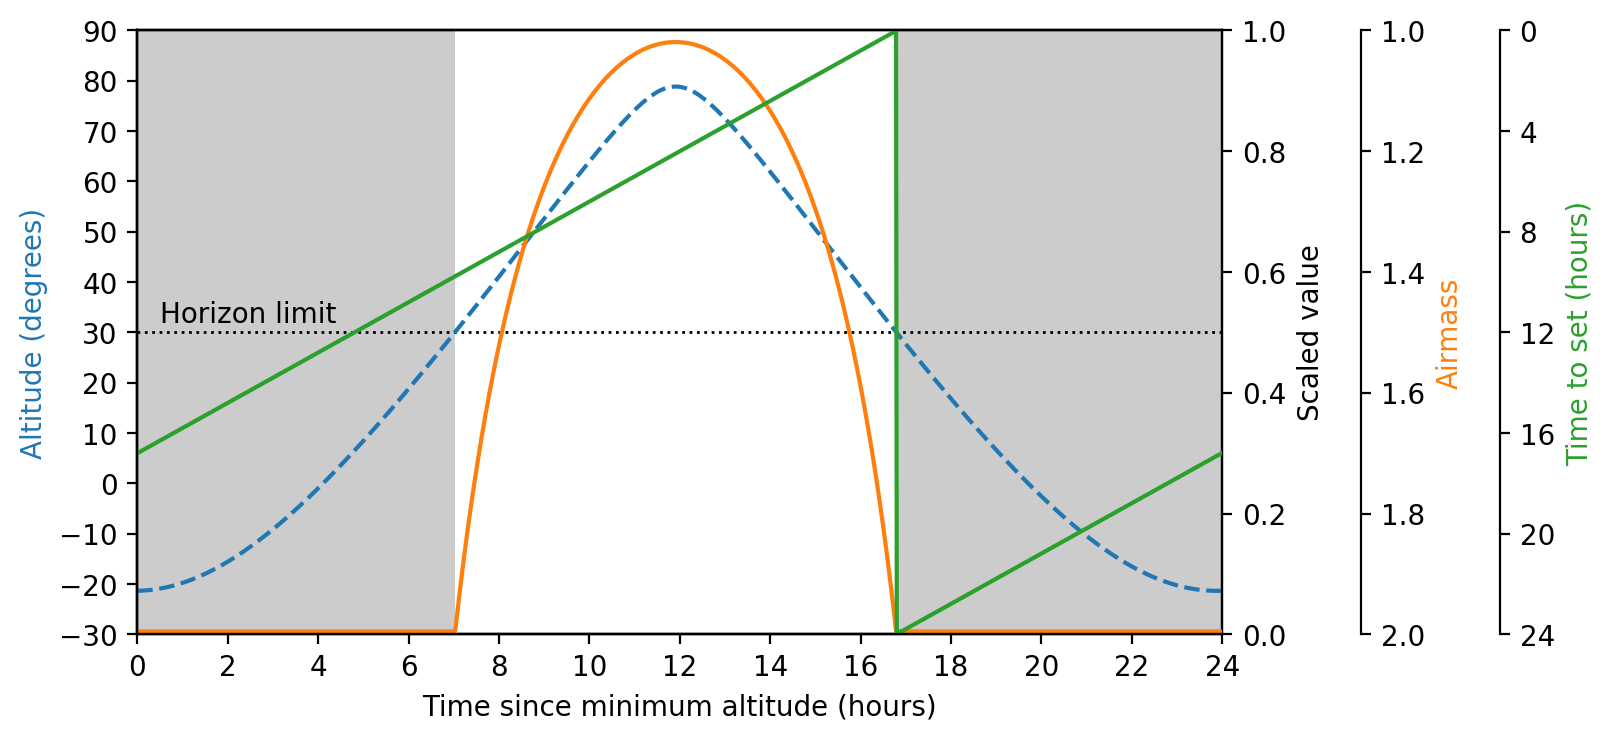
\includegraphics[width=\linewidth]{images/airmass-tts.png}
    \end{center}
    \caption[Plotting scaled airmass and time-to-set values for a target]{
        Plotting scaled airmass and time-to-set values for a target over 24 hours.
        The altitude of the target is shown by the \textcolorbf{NavyBlue}{blue} dashed line, and the \textcolorbf{Gray}{grey} regions show the times when the target is below the \SI{30}{\degree} horizon altitude limit (the black dotted line).
        The two tiebreak values are also plotted, scaled between 0 and 1: airmass (in \textcolorbf{Orange}{orange}) is set to 0 when the target is at airmass 2 or below, and the time-to-set (in \textcolorbf{Green}{green}) linearly increases to 1 until the target passes below the horizon and it is reset to 0.
    }\label{fig:airmass_tts}
\end{figure}

Just replacing airmass in the tiebreaker calculation with the time-to-set would not produce good results, as the telescope would be prioritised to observe the western horizon continuously (as by design targets that are just about to set have the highest scaled time-to-set values). As when including the skymap probability, a weighted combination of both airmass and time-to-set would be best in order to take both parameters into account. This new parameter, $Z$, can be considered using the equation
%
\begin{equation}
    Z = \frac{a}{a+t}~(2-X) + \frac{t}{a+t}~T,
    \label{eq:at_ratio}
\end{equation}
%
where again the weighting factors $a$ and $t$ describe the relative ratio between the airmass ($X$) and time-to-set ($T$) in the ratio $a$:$t$. \aref{fig:at_ratio} shows how different ratios produces different distributions: a ratio of 1:0 only considers the airmass, a ratio of 1:1 has to two equally weighted and a ratio of 0:1 only considers the time-to-set. As the ratio is increased in favour of time-to-set (i.e.\ $t$ is larger than $a$) the peak of the distribution shifts to the right, which will favour targets that are setting over those at the zenith. By using both airmass and time-to-set values in the tiebreaker formula the scheduler should prioritise observing targets that are about to set but are still at a reasonable airmass.

\begin{figure}[t]
    \begin{center}
        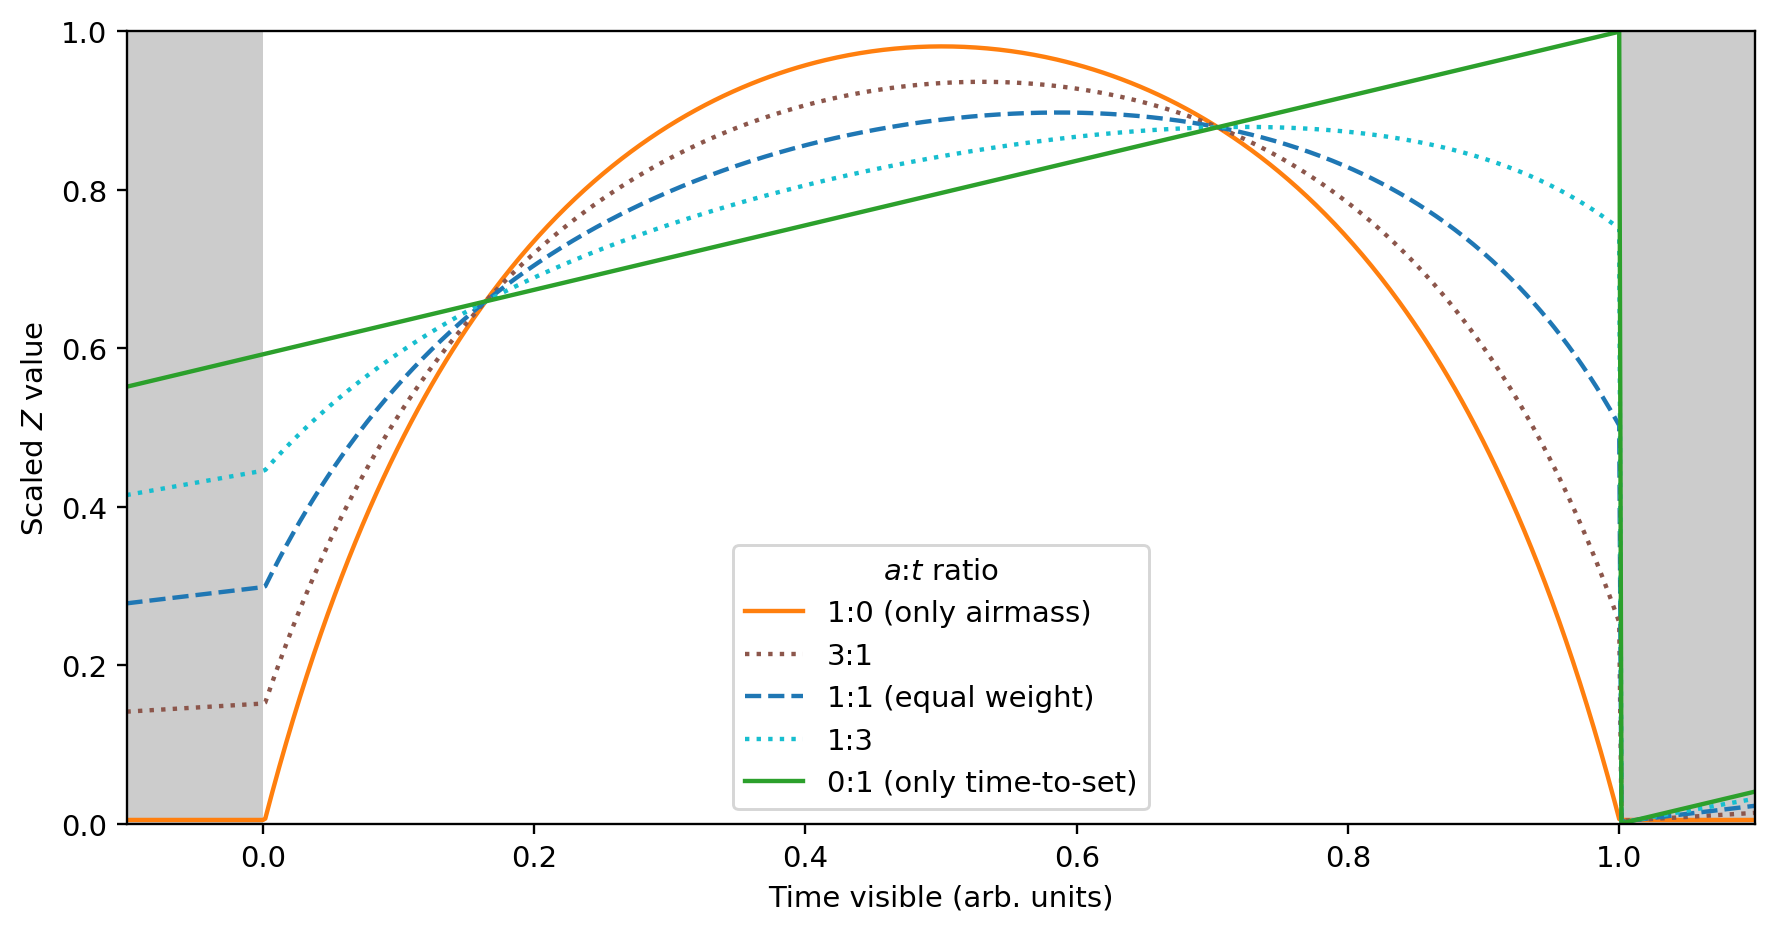
\includegraphics[width=\linewidth]{images/at_ratio.png}
    \end{center}
    \caption[Combining airmass and time-to-set values]{
        Combining airmass and time-to-set values in different ratios using \aref{eq:at_ratio} to create a new distribution. This plot uses the same target as \aref{fig:airmass_tts}, but focusing the $x$-axis on the time when the target is above the horizon.
    }\label{fig:at_ratio}
\end{figure}

\newpage

Previously, the scheduler tiebreak value $V$ was calculated using equation \aref{eq:wa_ratio} with just the tile weight ($W$) and the airmass ($X$). In order to determine how including the time-to-set ($T$) would affect the scheduler this equation can be rewritten as
%
\begin{equation}
    V = \frac{w}{w+a+t}~W + \frac{a}{w+a+t}~(2-X) + \frac{t}{w+a+t}~T,
    \label{eq:wat}
\end{equation}
%
where $w$, $a$ and $t$ are the relative weightings factors for the tile weight, airmass and time-to-set respectively (usually written in the form $w$:$a$:$t$). Using this equation a series of simulations were carried out using the GOTO scheduling code to determine optimal values for $w$, $a$ and $t$, as described in the \aref{sec:scheduler_sims}. Ultimately a ratio of 10:1:0 was selected; by setting $t=0$ the time-to-set value is ignored, as it was found to only hinder the scheduler performance. This is why \aref{eq:tiebreak} in \aref{sec:breaking_ties} only includes the tile weight and airmass values.

\end{colsection}

% ########################################

\section{Scheduler simulations}
\label{sec:scheduler_sims}

% ~~~~~~~~~~~~~~~~~~~~

\begin{colsection}

When the scheduling functions described in the previous sections were written, it was not clear how best to combine the selected parameters (tile weight, airmass and time-to-set) to create a single tiebreak value. In order to examine how different weightings of the three parameters affected the scheduler performance, a series of simulations were carried out. These simulations, and their results, are described in this section.

\end{colsection}

% ~~~~~~~~~~~~~~~~~~~~

\subsection{Simulating GOTO}
\label{sec:goto_sims}
\begin{colsection}

The G-TeCS control system described in \aref{chap:gtecs} and \aref{chap:autonomous} contains all of the code used to operate the GOTO telescope, as well as test code down to the level of the individual daemons and hardware units. This makes it possible to simulate, for example, the camera daemon taking exposures using fake hardware code that waits in real time until the exposure time is completed (plus some readout time) and then creates a blank FITS image file with all of the expected header information. On top of this the real pilot can run without knowing these daemons are fake, and the real sentinel daemon can add real or simulated events into a copy of the observation database for the real scheduler to choose between. In this way the entire control system can be run without connecting it to any real hardware.

However, the fully-featured test suite described above is not necessary for the simulations described in this section: ideally they would run faster than real time, and it is not necessary to simulate the full hardware system down to fake images being created, but the intention is still to model the response of the real control system as much as possible. For these simulations anything below the pilot (i.e.\ the hardware daemons, as shown in \aref{fig:flow}) is abstracted away, and the pilot itself is replaced by a new specialised script simply called the fake pilot. This mirrors the real code described in \aref{sec:pilot} in most ways, however there are several important simplifications:

\begin{itemize}
    \item The fake pilot does not call the scheduler daemon in order to find what pointing to observe, but instead imports and runs the scheduling functions itself. This was the original way the pilot ran before the scheduler was split into a separate daemon, as described in \aref{sec:scheduler}.
    \item The fake pilot does not include the full conditions monitoring system described in \aref{sec:conditions}. The \code{check\_conditions} routine still exists in order to stop observations when the Sun has risen, but is just a single function check. Code was written to simulate weather closing the dome using random Gaussian processes, however for the scheduling simulations described here only a single night of observations is considered, and including random weather effects in the simulations only distracted from their purpose to model the scheduler response.
    \item The night marshal and any observing tasks other than actually observing the scheduler target (e.g.\ autofocusing) have been removed from the fake pilot. Observations start immediately after sunset and continue to sunrise, and then when the dome is closed the pilot loop continues until the simulation has completed.
    \item While the real pilot works using loops that sleep until a given time has passed, the fake pilot contains an internal time which is increased for each `step' in the simulation. At each step the script checks the scheduler using the normal commands. One important factor in speeding the simulations up is to increase this step size, up to the point that each observation takes a single step. This means that at each step the pilot will observe a new target, and increase the internal simulation time by the appropriate amount. If, for example, the target pointing asks for three \SI{60}{\second} exposures the simulations would increase by 3 minutes, plus extra time for readout and slewing to the target before the exposures start.
\end{itemize}

\newpage

\end{colsection}

% ~~~~~~~~~~~~~~~~~~~~

\subsection{Simulation results}
\label{sec:scheduler_sim_results}
\begin{colsection}

A series of simulations using the fake pilot code described above were carried out in order to find optimal values for the weights ($w$, $a$ and $t$) given in \aref{eq:wat}, and to see how the telescope response changes depending on the values used.

It should be noted that these simulations were carried out in 2016, early in the development of G-TeCS and before the first GOTO telescope had been commissioned on La Palma. They therefore included assumptions for values such as the field of view of the telescope (affecting the tile size), mount slew speed and readout time. In addition, most of the code to handle gravitational-wave skymaps detailed in \aref{chap:alerts} had not yet been written and the event follow-up strategy had not been fully defined.

In order to run the simulations, a selection of model skymaps from the LIGO First Two Years project \citep{First2Years} were manually processed to generate a series of tiled pointings, which were then added to the observation database. The fake pilot script was then run to simulate one night of observations using set values for the $w$:$a$:$t$ ratio. Once completed the tiles observed were recorded, and then the database was reset, the ratio changed and the simulations repeated.

Two metrics were used to judge the effectiveness of the scheduler response: the mean airmass of each tile when observed, and the fraction of the skymap probability covered (i.e.\ the total contained probability within all observed tiles). As simulated skymaps were being used the location of the source of the gravitational-wave signal was known, so it was possible to record if the tile containing the source was observed or not. However, for these simulations the overall response, in terms of skymap coverage, was deemed a better indicator of the scheduler performance than just if the source was observed or not (for example, the source might not have even been visible from La Palma). The later, more advanced simulations described in \aref{chap:multiscope} go into more detail about the source location and the probability that the source position is observed.

\newpage

\end{colsection}

% ~~~~~~~~~~~~~~~~~~~~

\subsection{Analysis of simulation results}
\label{sec:scheduler_sim_analysis}
\begin{colsection}

\begin{figure}[t]
    \begin{center}
        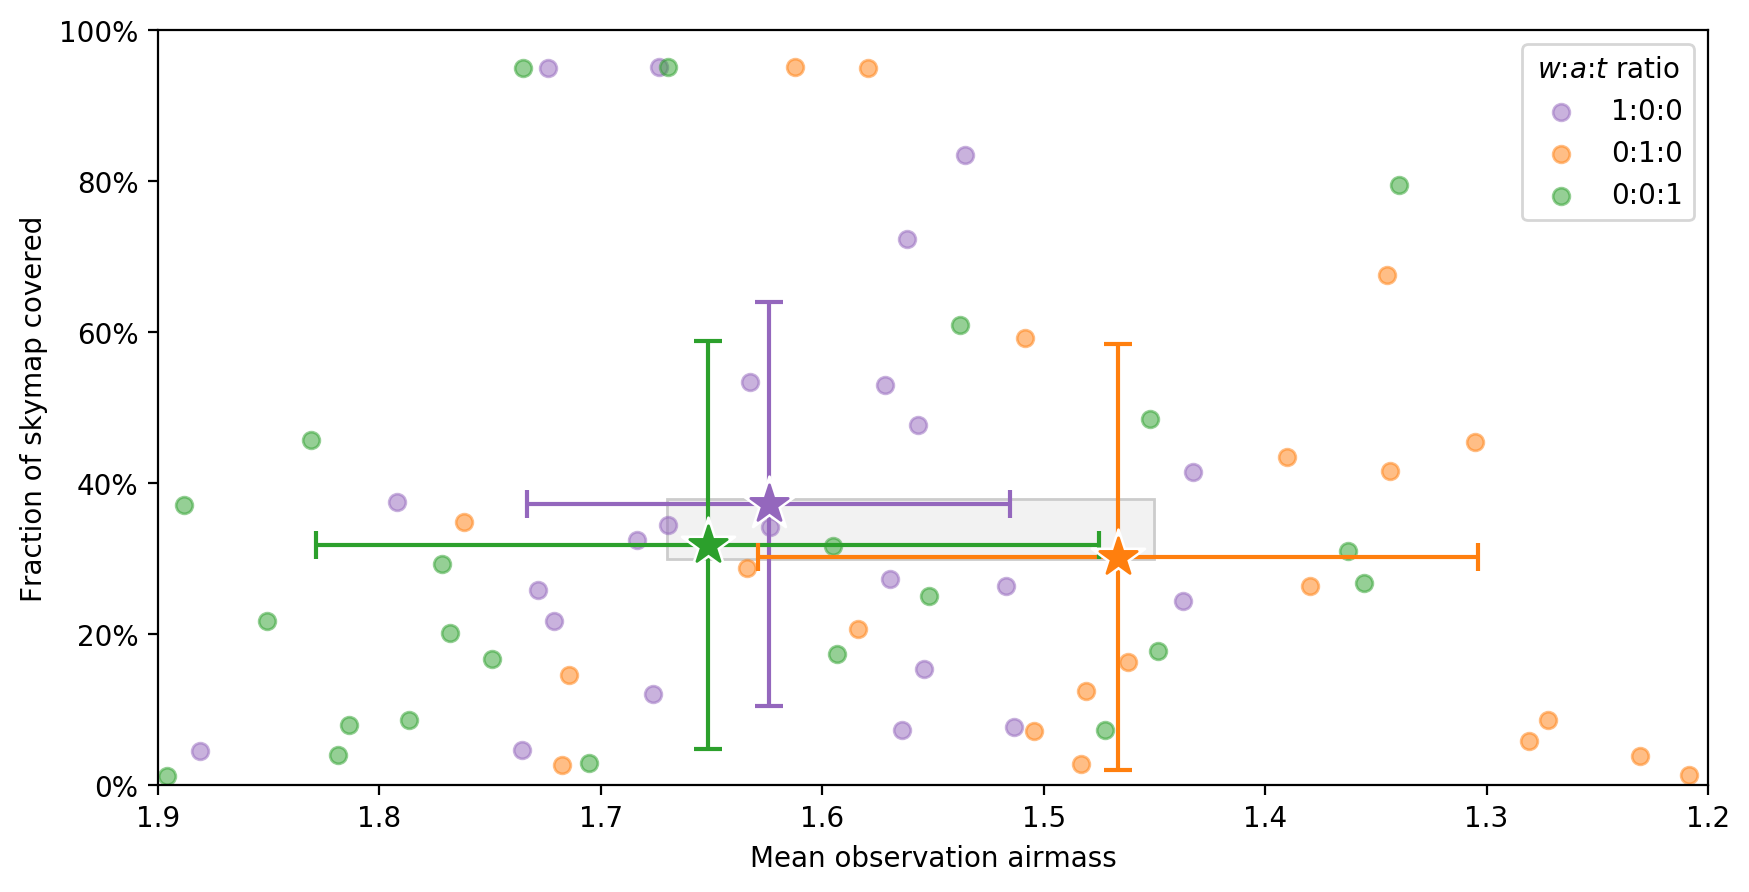
\includegraphics[width=\linewidth]{images/sched_sim1.png}
    \end{center}
    \caption[Skymap coverage verses mean airmass for different $w$:$a$:$t$ ratios]{
        The fraction of the event skymap covered verses the mean observation airmass for three different $w$:$a$:$t$ ratios: 1:0:0 (\textcolorbf{Purple}{purple}), 0:1:0 (\textcolorbf{Orange}{orange}) and 0:0:1 (\textcolorbf{Green}{green}). Each point represents a simulation using one of the First 2 Year skymaps. The stars show the average position for each ratio, with the error bars showing the standard deviation. The shaded region shows the area of \aref{fig:scheduler_sim_results2}.
    }\label{fig:scheduler_sim_results1}
\end{figure}

The simulation results for three different ratios are plotted in \aref{fig:scheduler_sim_results1}. Each coloured point represents a single simulation of a night observing a single skymap. There is a large range of results: some simulations covered close to 100\% of the skymap while others covered almost none. Only simulations that included observing at least one skymap tile are included, otherwise the mean observed airmass would be undefined. The stars show the average position for each $w$:$a$:$t$ ratio. Although the errors are clearly large, some distributors are clear. For example, the 0:1:0 ratio (only including the airmass weighting) on average produces a better mean airmass than the others, which would be expected. Likewise the 1:0:0 case (only including the tile weight) on average results in a slightly higher fraction of the skymap being observed.

\begin{figure}[t]
    \begin{center}
        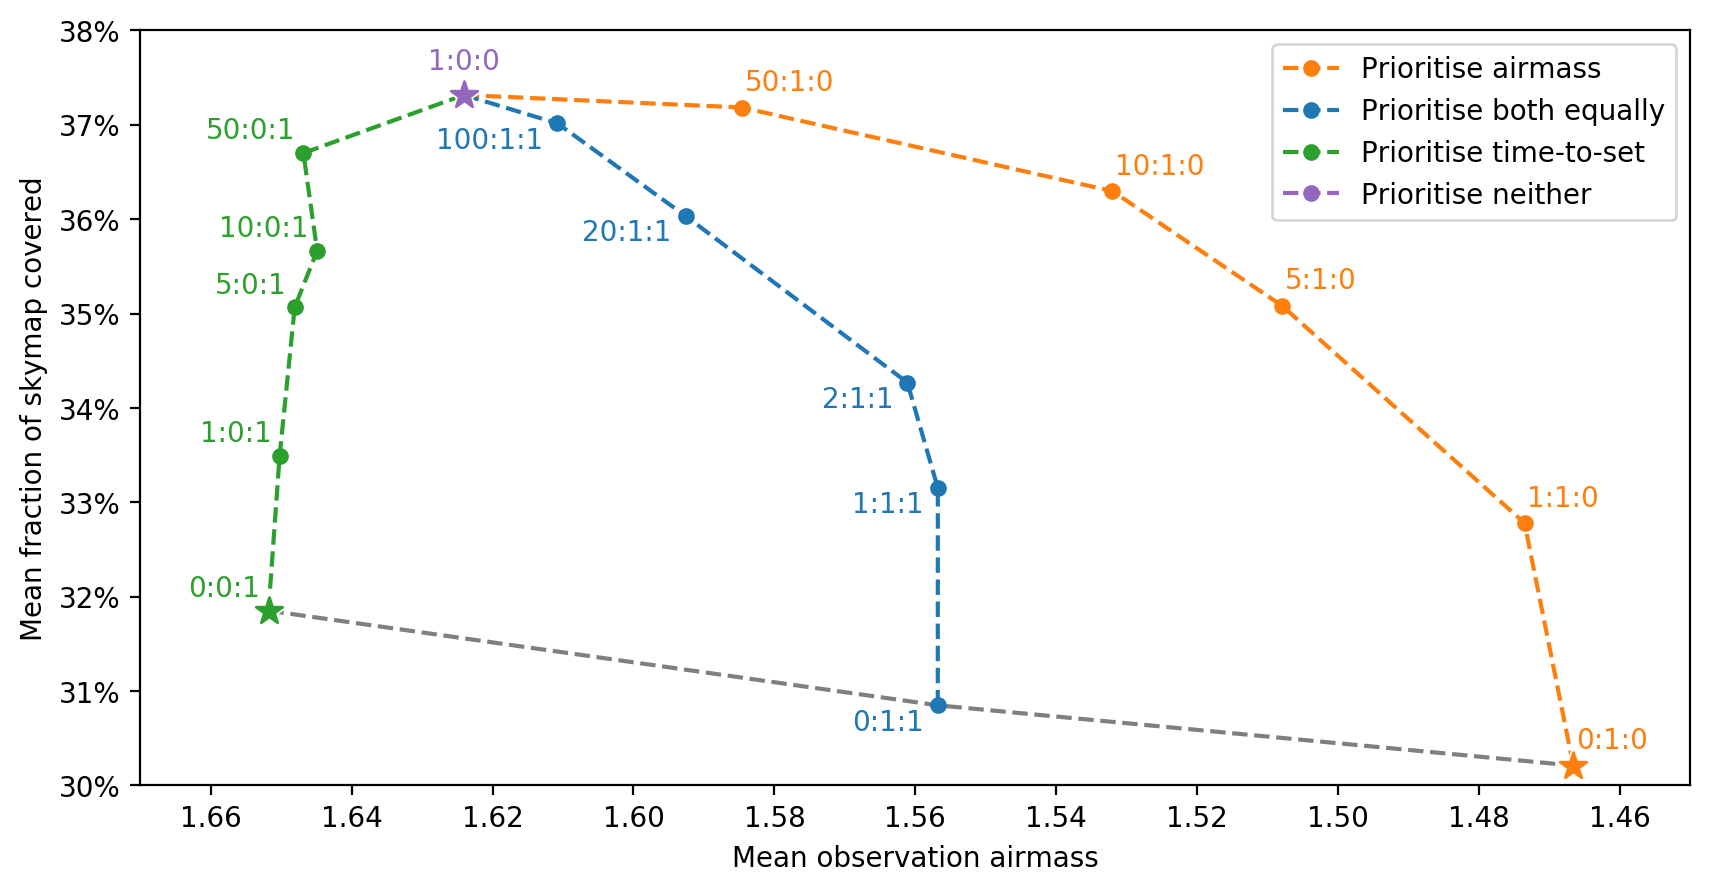
\includegraphics[width=\linewidth]{images/sched_sim2.png}
    \end{center}
    \caption[Scheduler simulation results for different $w$:$a$:$t$ ratios]{
        The fraction of the event skymap covered verses airmass for multiple different $w$:$a$:$t$ ratios. Each point here shows the average over multiple simulations of different skymaps, and the ratios shown by stars are the same as plotted in \aref{fig:scheduler_sim_results1}. The dashed coloured lines join results with the same $a$:$t$ ratio; 1:0 in \textcolorbf{Orange}{orange}, 1:1 in \textcolorbf{NavyBlue}{blue}, and 0:1 in \textcolorbf{Green}{green}; and the \textcolorbf{Gray}{grey} dashed line joins ratios with $w=0$.
    }\label{fig:scheduler_sim_results2}
\end{figure}

Simulations were repeated for multiple different $w$:$a$:$t$ ratios, and the averages for each are plotted in in \aref{fig:scheduler_sim_results2}. This plot shows that, while there is a lot of underlying scatter between different skymaps as shown in \aref{fig:scheduler_sim_results1}, the mean positions for each ratio follow remarkably smooth trends (error bars are omitted from \aref{fig:scheduler_sim_results2} as they would spread off the page in both axes). For example, the higher the tile weight value $w$ relative to the other two parameters consistently increases the mean fraction of the skymap covered, however this is at a cost to the mean airmass of the observations.

Changing the relative ratios of airmass to time-to-set (from 1:0 through 1:1 to 0:1) shows an unexpected result. It is true the observed airmasses would be lower as less weight is put on the airmass parameter, however it was intended that introducing the time-to-set parameter would compensate by catching more setting tiles that would be missed by purely looking around the zenith, and therefore the skymap fraction covered would be higher. This is true if the tile weight is not included as a factor, as seen by the grey 0:0:1--1:0:0 line at the bottom of \aref{fig:scheduler_sim_results2}: when only airmass is considered (in the 0:1:0 case) the results produce the best average airmass per observation but the worse skymap coverage, and on the other hand only considering time-to-set (0:0:1) results in worse airmasses but better coverage. However, when the tile weight value $w$ is included this trend is counteracted, to the extent that the 50:0:1 point has both a higher mean airmass and a lower fraction of the skymap covered than the 50:1:0 point. In fact, based on the results which do not include the airmass parameter (the green line on the left of \aref{fig:scheduler_sim_results2}) the time-to-set value just suppresses the fraction of the skymap observed, while making almost no difference to the mean airmass.

The optimal scheduler result would, on average, produce the highest possible skymap coverage for the lowest average airmass. This would fall in the top-right region of \aref{fig:scheduler_sim_results2}. Based on these simulation results the best solution is to ignore the time-to-set value, and as described previously in \aref{sec:breaking_ties} the G-TeCS scheduler has been operating with a ratio of 10:1:0.

\end{colsection}

% ~~~~~~~~~~~~~~~~~~~~

\subsection{Further simulations}
\label{sec:scheduler_sim_future}
\begin{colsection}

The conclusions from these scheduler simulations are not unreasonable if all that is needed is a one-size-fits-all set of weights that are hard-coded into the scheduler, as used by the current G-TeCS system. However, future work on these simulations should look in detail at other trends that might be hidden in the averages. For example, different $w$:$a$:$t$ ratios might be better suited for large skymaps versus smaller ones, or in cases where the whole skymap is visible at once compared to it slowly rising above the horizon during the night.

Although the time-to-set value seemed to only hinder the scheduler, other possible parameters could be considered. One idea is to convert time-to-set to time-visible, by including not only the time when the target sets below the horizon but also the time that the Sun rises. The existing time-to-set ratio prioritises observing targets later in the night when they are about to set, whereas airmass prioritises tiles near the zenith. Neither however considers the time remaining in the night, and while this is the same for every target including it as a factor in the scheduler could be a relatively-straightforward way to attempt to prioritise observations in the limited time available.

As mentioned previously, the simulations presented in this section were carried out before a lot of the G-TeCS code was finalised. Therefore it would also make sense to revisit the scheduler simulations with the newer simulation code, as used by the simulations in \aref{chap:multiscope}, in order to confirm if the 10:1:0 ratio is still found to be the best case. This would also allow the real parameters from the commissioned telescope to be included. When the next four unit telescopes are added to GOTO the effective field of view will be doubled, and the results in this section based on the 4-UT telescope might not necessarily be the same in the 8-UT case.

Finally, GOTO is ultimately planned to expand to multiple telescopes at several sites, as described in \aref{sec:goto_expansion}. Adapting the scheduling system described into this chapter to deal with multiple telescopes will be a major future project, which is considered in more detail in \aref{chap:multiscope}.

\end{colsection}

% ########################################

\section{Summary and Conclusions}
\label{sec:scheduling_conclusion}

% ~~~~~~~~~~~~~~~~~~~~

\begin{colsection}

In this chapter I described how the G-TeCS automated scheduling system decides which pointings to observe.

The scheduler daemon is one of the autonomous support daemons as defined in \aref{chap:autonomous}. It has the task of taking the queue of possible targets from the observation database and sorting them based on several parameters to determine which is the highest priority. First each pointing is tested using a series of physical constraints to remove any which are invalid. The queue sorting then depends on the properties of each pointing: its rank, the number of times it has already been observed, whether it is defined as a target of opportunity or not. If there are still multiple pointings in the same position in the queue then a final tiebreaker value is calculated to chose between them, based on the skymap tile weighting (defined in \aref{chap:tiling}) and target airmass.

Determining how to calculate the tiebreaker and which parameters to base it on required a series of simulations of GOTO observations, to see how the choice of parameter weightings affected which pointings were observed. These simulations showed that a 10:1 ratio of tile weight to scaled airmass was closest to the preferred outcome, and that the introduction of a third parameter, time-to-set, could not improve on this. GOTO has been observing successfully using this ratio ever since. However, since those simulations were carried out further development of the control system and simulation code means that it would be worth revisiting them to see if the conclusions still hold.

\end{colsection}

% ########################################
